%%%%%%%%%%%%%%%%%%%%%%%%%%%%%%%%%%%%%%%%%
% Practical 2 CS181
%%%%%%%%%%%%%%%%%%%%%%%%%%%%%%%%%%%%%%%%%

%----------------------------------------------------------------------------------------
%	BASIC PACKAGES AND DOCUMENT CONFIGURATIONS
%----------------------------------------------------------------------------------------

\documentclass{article}

\usepackage[version=3]{mhchem} % Package for chemical equation typesetting
\usepackage{siunitx}  				 % Provides the \SI{}{} and \si{} command for typesetting SI units
\usepackage{graphicx} 				 % Required for the inclusion of images
\usepackage{natbib}   				 % Required to change bibliography style to APA
\usepackage{amsmath}  				 % Required for some math elements 
\usepackage[left=2.2cm,top=1.6cm,right=2.0cm,nohead,nofoot]{geometry} % Set margins
\usepackage[section]{placeins}
\usepackage{amsfonts}
\usepackage{booktabs}
\usepackage{array}
\usepackage{hyperref}
\setlength{\footskip}{20pt}  % Distance of page number to text
\setlength\parindent{0pt} % Removes all indentation from paragraphs
\renewcommand{\labelenumi}{\alph{enumi}.} % Make numbering in the enumerate environment by letter rather than number (e.g. section 6)

%\usepackage{times} % Uncomment to use the Times New Roman font

%----------------------------------------------------------------------------------------
%	REPORT HEADER
%----------------------------------------------------------------------------------------
\title{\vspace{-0.5cm}Stuff}
\title{Malware Classification} % Title

\author{Authors: Taylor Names, Samuel Kaplan and David Castineira} % Author name
\date{\vspace{-5ex}}  % Remove date
\begin{document}

\maketitle % Insert the title, author and date


%----------------------------------------------------------------------------------------
%	SECTION: INTRODUCTION
%----------------------------------------------------------------------------------------

\section*{Introduction}

The fundamental objective of this project is to use machine learning techniques to classify malicious software using executable files collected from people's computers. A total of 14 known malware classes are being considered (plus one additional class i.e., None, for executables that are not malware at all). For training purposes a total of 3086  documents (.xml files) were made available. Our ultimate goal is to make predictions for 3724 executables documents (and that represent our test set). 


%----------------------------------------------------------------------------------------
%	SECTION: TECHNICAL APPROACH
%----------------------------------------------------------------------------------------

\section{Technical Approach}

Our approach for this problem can be divided into three different efforts or initiatives: 

\begin{description}

\item[1.1 Preliminary Data Analysis:] \hfill \\

The dataset posed a number of machine learning challenges. It contained a relatively small number of total data points. More problematic, there were a very small number of training points for each class. Some classes only had a few dozen points to train on. This made the variance of any classification technique fairly large.

The amount of information in each file was limited as well. Commercial antivirus software uses a much wider and deeper set of techniques. The provided input contained only very high level calls made by the process and some miscellaneous information. Looking at the smallest files was a good way to begin analysis since there was less information total to understand. There was a notable dearth of information in some files. 

For instance, comparing file ��61222ec5...41cc437.Agent.xml and file ��a4251cfc8...2530c56d.None.xml, there is almost no difference! One is a virus and one is not, but besides capitalization, process ids, times, and one or two filenames, they were completely the same. None of these differences seemed significant in any way. It is not a good technique to be basing decisions on filenames or process ids (or slight variations in timing) since these things easily change without the underlying class of the process changing.
Moreover, the opposite problem occurred, the same class of virus could generate files that looked very different. This is less of a problem since if there is some common factor then the algorithm should identify it. However, a large file will have a lot of extraneous information.

\item[1.2 Feature engineering:] \hfill \\

One of our initial attempts for feature extraction was to use the so-called Term-Document Matrix technique [1]. Within this technique, which was originally developed in the field of Information Retrieval,  vector spaces are used for constructing mathematical representations of documents, words and any other type of textual units. Basic geometrical concepts, such as distances, angles and projections, are then used to assess difference and similarity degrees among the units of analysis under consideration, which are modeled by means of vectors in the given vector space. This approach is commonly used in natural language modeling. Nevertheless for this particular exercise of malware detection from .xml files the resulting matrix sizes were too large (i.e., more than 100,000 features were generated). This was probably due to the need of accommodating a large number word occurrences, co-occurrences, overlaps, etc... from documents that are not really natural language representations. We decided not to pursue this path after realizing that the number of resulting features was much larger than the number of samples (documents) available for training. 

To test the quality of features, sklearn's support vector classification was used. This classifier was chosen by experiment. Looking through the variety of sklearn's classifiers, SVC was fast and high quality. While the final product used gradient boosted trees, svc allowed for an estimate of feature quality. 

Since each XML file contains enough information to create a nearly infinite amount of features, we had to narrow our focus. Without having much background in spyware detection, we focused on the areas suggested by the teaching staff. In the data description on the Kaggle site, the course staff expressed the importance of processes and calls occurring inside the all\_section category. Also, in the sample code, the staff provided a process to extract counts for different call types. We decided to extract features that included counts of all types of calls (inside and outside of the all\_section category) as well as counts of first and last calls within the all\_section category. Furthermore, the totals of calls inside and outside of all\_section were included as features. Finally, due to a suggestion by a TF on piazza, we pursued the extraction of the bigrams of all calls within the all\_section category. In the end, we extracted $2,669$ distinct features for each XML file. The following feature engineering methods were also explored:

- N-grams greater than two: N-grams greater than two, where each word was a function call, provided worse results than bigrams. Take sequence ABCABD. 3-grams chunks it to ABC, ABD. There�'s nothing connecting ABC with ABD even though they are mutually dependent. It seems like it would be better to generate every 2-gram in addition to every 3-gram. Yet, these significantly increase the number of features. While there is some computational limit to this, the bigger issue is that it reduced the quality of the classification. It seems as though having too many features adds a lot of noise and promotes over fitting.

- Recursive N-grams: The features used to generate the submission predictions only dealt with top level calls. Adding in the subcalls did not improve the predictions. Adding the subcalls probably obfuscated the more general structure of the program. 

- Total size: Adding all the size attributes also did not generate any better results. The size doesn't really matter since the same virus (or not virus) can very significantly.

- Attributes: Counting the number of attributes increases the amount of information available. However, it suffers from the same problems of n-grams. Attributes add noise, don't provide that much information and they promote overfitting.

\item[1.3 Classification:] \hfill \\

Two techniques (Neural Networks and Boosted Trees) were considered here for classification: 
 
\item[\hspace{0.75cm}$\bullet$ Gradient Boosted Trees:] Gradient boosted trees is a non-parametric technique that combines several 'weak' decision tree models trained by iteratively improving on residuals from sequentially trained trees. Gradient boosted trees are a particularly attractive method due to the ability to model non-linear behavior, feature interactions, and skewed features without transformation. Also, as an ensemble approach of many 'weak' learners, gradient boosted trees can be quite proficient in avoiding overfitting. The python package XGBoost [2] was used for the gradient boosted trees model due to its speed and parallelization.
As the number of features including bigrams was quite large, hyperparameter tuning was performed on a subset of 50 percent of the training set. The hyperparameters tuned in a 3-fold grid search cross-validation were the following:

\item[\hspace{1.5cm}$\cdot$ max\_depth:] maximum depth of each boosted tree $[8,10,12]$
\item[\hspace{1.5cm}$\cdot$ colsample\_bytree:] Proportion of features used in each boosted tree $[0.6,0.75,1]$
\item[\hspace{1.5cm}$\cdot$ subsample:] Proportion of total samples considered for each boosted tree $[0.6,0.8,1]$

Increasing the value of each of these hyperparameters leads to a higher variance/lower bias model. The optimal hyperparameters were selected as they provided a balanced model in variance and bias. The optimal parameters for 'max\_depth', 'colsample\_bytree', and 'subsample' were found to be 8, 0.75 and 0.8 respectively.

\item[\hspace{0.75cm}$\bullet$ Artificial Neural Networks:] Artificial neural networks are typically presented as systems of interconnected "neurons" which exchange messages between each other. The connections have numeric weights that can be tuned based on experience, making neural nets adaptive to inputs and capable of learning. For classification exercises the softmax function is often implemented at the final layer of a network. The Matlab Neural Networks Toolbox [3] was used for this study. Several network architectures were considered (mainly by varying the number of hidden layers and the number of neurons on each hidden layer). The training files acted as inputs to a neural network, and the respective target for each was a 15-element class vector with a 1 in the position of the associated malware, 1, 2, 3 up to 15 (one-hot encoding). Notice that once the network architecture was defined, training samples were automatically subdivided into training, validation and test sets. The training set was used to teach the network. Training continued as long as the network continues improving on the validation set. The test subset is supposed to provide a completely independent measure of network accuracy, and it was used as an estimate of the classification accuracy for the real test set.  


\end{description}

 
%----------------------------------------------------------------------------------------
%	SECTION: RESULTS and DISCUSSION
%----------------------------------------------------------------------------------------

\section{Results and Discussion}

ANN classification accuracies (estimated using subsets of the training data as discussed earlier) was consistently very high (around 0.9), but that same classification power went down (to 0.6-0.7) once the same network was implemented on the real test set on Kaggle. While there could be several explanations for this problem, we attributed it to the fact that ANN may be overfitting the data given the limited sample size for training (and a much larger test set size). This is clearly seen in Figure 1 for one of our ANN runs with 1 hidden layer, 10 hidden neurons and equal-size partitioning of the training set (into training, validation and test subsets). This plot basically displays the errors for different epochs on the left panel (one curve for each subset) and the resulting Receiver Operating Characteristic (ROC) curves on the right panel. The resulting classification accuracy from this model was 0.9, which was really high. However, the real test set on Kaggle did not show the same level of accuracy unfortunately. In fact the error curves seem to indicate overfitting (as the error on both validation and test subsets are much higher than errors on the training set).\\


\begin{figure}[!h]
\begin{center}
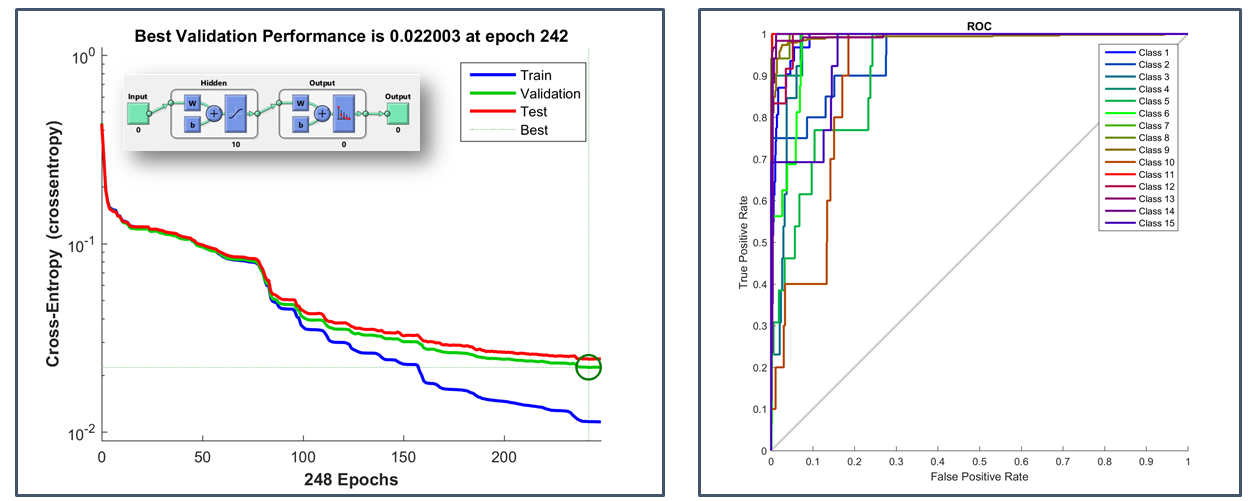
\includegraphics[scale=0.45]{ANN_plot} % Include the image placeholder.png
\end{center}
\vspace*{-5mm} % Space between figure and captio
\caption{ Cross-entropy and ROC curves resulting from classification of the training set using ANN.}
\label{fig:ANN_plot}
\end{figure}

Therefore we decided to focus our modeling efforts on the Gradient Boosted Trees as they provided higher classification accuracies for the problem at hand, while probably minimizing the negative effects of overfitting that we observed with ANNs. Our analysis using XGBoost was broken down into three iterations. First, the model was trained utilizing the original "count" features without the use of bigrams. Hyperparameters were chosen through a 3-fold cross validation procedure. The result was very positive, as with a mere 106 features, we were achieving around 82\% accuracy as seen in Table~\ref{tab:CatAccuracy} . The second iteration included all occuring bigrams in the training set. Initially, trained our model using the hyperparameters from the previous iteration. Once again, we saw a significant improvment with an accuracy of nearly 83\%. Finally, we performed hyperparameter tuning through cross validation and the result was nearly identical.\\

During this process, we noticed a discrepancy between the cross-validation score (which hovered around 90\% accuracy) and the score on the public leaderboard (83\% accuracy). Despite the cross validation procedure, our model was overfitting. Possible explanations for this overfitting could be due to the small training set size compared to the test set, or an unbalanced class proportions between the training and test sets.\\

An analysis of the confusion matrix of our final model shed some light on where our model was misclassifying. The confusion matrix is shown in n Figure~\ref{fig:confusion_matrix}. The model was misclassifying a significant proportion of malware belonging to the Zbot, Virut, and Agent classes as "None". To improve the classification accuracy, further analysis could be completed to help distinguish between the "None" class from the previously mentioned classes. \\

Finally, in an attempt to further improve our score without additional model training, we chose to create an ensemble of models. The predictions from three of the best scoring and independently generated models were combined using a simple majority vote. Making this minor addition yielded a significant improvement in our accuracy score as seen in Table~\ref{tab:CatAccuracy}. \\


\begin{table}[!h]
\begin{center}
\begin{tabular}{ c c c } \toprule
    {$Model$} & {$Model Description$} & {Accuracy - Test} \\ \midrule
		
    1  & {XGboost $106$ features: } &  0.81947  \\
    2  & {XGboost, $2669$ features} &  0.82947  \\
    3  & {XGboost, $2669$ features (CV)} &  0.82895  \\ 
    4  & {XGboost (Majority Vote): } &  0.83316  \\\bottomrule
\end{tabular}
\end{center}
\caption{Categorization accuracy for different supervised learning models implemented in this project.}
\label{tab:CatAccuracy}
\end{table}

 

\begin{figure}[!h]
\begin{center}
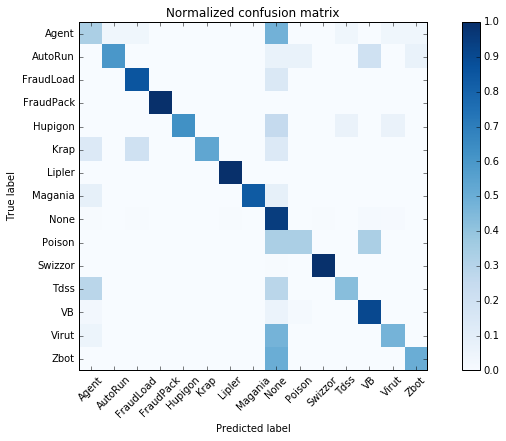
\includegraphics[scale=0.55]{confusion_matrix} % Include the image placeholder.png
\end{center}
\vspace*{-0mm} % Space between figure and captio
\caption{Confusion matrix.}
\label{fig:confusion_matrix}
\end{figure}

%----------------------------------------------------------------------------------------
%	BIBLIOGRAPHY
%----------------------------------------------------------------------------------------
\section*{References}
\fontsize{7pt}{7pt}\selectfont
\begin{itemize}
	\item {[1] Text Mining with Matlab (R.E. Banchs, Springer 2013)}
	\item {[2] XGBoost - https:\/\/github.com/dmlc/xgboost}
  \item {[3] Matlab, Neural Network toolbox (http:\/\/www.mathworks.com/help\/\nnet\/)}
\end{itemize}

%----------------------------------------------------------------------------------------
%	APPENDIX
%----------------------------------------------------------------------------------------
\section*{Appendix}
\fontsize{7pt}{7pt}\selectfont
All code from this practical can be found at the following Google Drive link: \\ \\ \url{https://drive.google.com/folderview?id=0B0e1_K8CvqynSWJuenRUdFRJN1U&usp=sharing} \\ \\



%----------------------------------------------------------------------------------------


\end{document}